% Appendix Template

\chapter{String Interpolation Grammar} % Main appendix title

\label{app:stringInterp} % Change X to a consecutive letter; for referencing this appendix elsewhere, use \ref{AppendixX}

\section{Original definition} \label{app:stringInterp:default}
\lstinputlisting[language=RascalGrammar, caption={A simple string-interpolation language as a Rascal grammar}]{Code/grammars/stringInterp/original.grammar}

\subsection{Simplified without priority} \label{app:stringInterp:simple}
\lstinputlisting[language=RascalGrammar, caption={The plain grammar with priority removal}]{Code/grammars/stringInterp/plain.grammar}

\pagebreak
\subsection{Strongly Regular} \label{app:stringInterp:stronglyregular}
\lstinputlisting[language=RascalGrammar, caption={The strongly regular approximation of the original grammar}]{Code/grammars/stringInterp/stronglyregular.grammar}

\subsection{NFA for strongly regular StringLiteral}
\begin{figure}[h!]
	\centering
	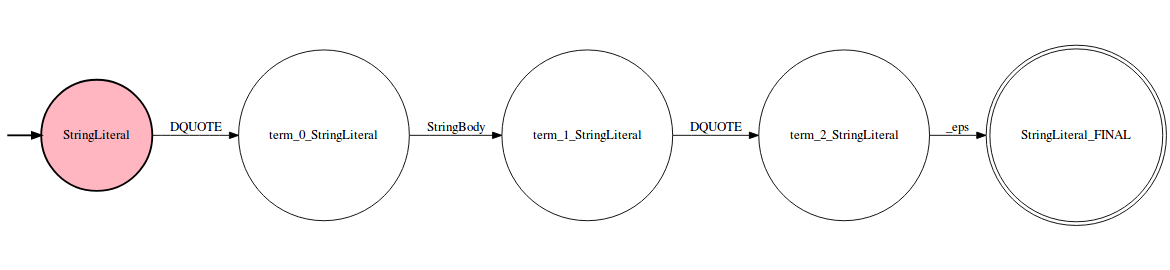
\includegraphics[width=\textwidth, keepaspectratio]{Figures/String_nfa_stringliteral.png}
	\decoRule
 	\caption[NFA for StringLiteral]{The NFA for StringLiteral, produced from the strongly regular approximation}
 	\label{fig:stringInterp:NFA:StringLiteral}
\end{figure}


\subsection{DFA for strongly regular StringLiteral}
\begin{figure}[h]
	\centering
	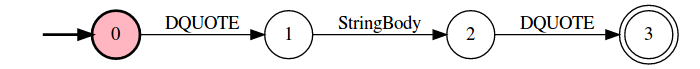
\includegraphics[width=\textwidth, keepaspectratio]{Figures/String_dfa_stringliteral.png}
	\decoRule
 	\caption[DFA for StringLiteral]{The DFA for StringLiteral, produced from the strongly regular approximation}
 	\label{fig:stringInterp:DFA:StringLiteral}
\end{figure}

\pagebreak\subsection{Results of generated highlighter}
\begin{figure}[h!]
	\centering
	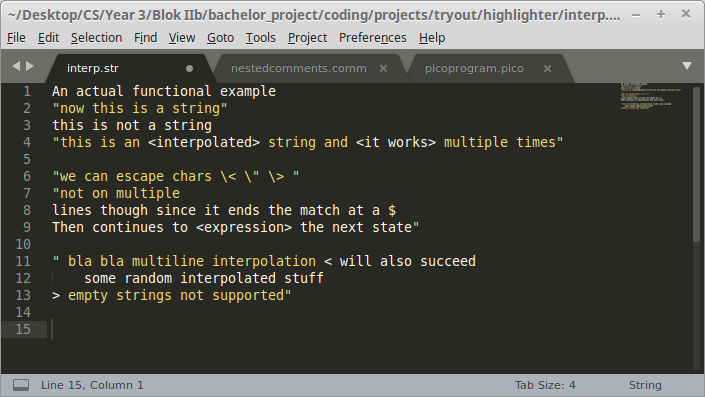
\includegraphics[width=\textwidth, keepaspectratio]{Figures/highlightShots/string_generated.png}
	\decoRule
 	\caption[Generated highlighter results for StringInterpolation grammar]{Results of the highlighter generated for this grammar}
 	\label{fig:stringInterp:highlighter:generated}
\end{figure}

\subsection{Results of hand-written highlighter}
\begin{figure}[h!]
	\centering
	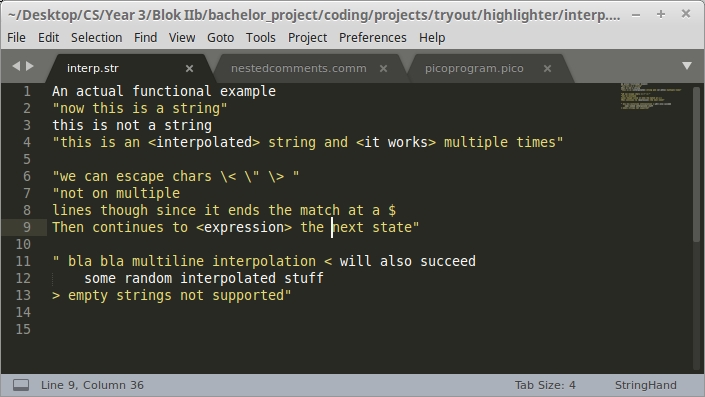
\includegraphics[width=\textwidth, keepaspectratio]{Figures/highlightShots/string_handwritten.png}
	\decoRule
 	\caption[Hand-written highlighter results for StringInterpolation grammar]{Results of a handwritten highlighter for this grammar}
 	\label{fig:stringInterp:highlighter:written}
\end{figure}